% !TEX TS-program = knitr
\documentclass[handout]{beamer}\usepackage{graphicx, color}
%% maxwidth is the original width if it is less than linewidth
%% otherwise use linewidth (to make sure the graphics do not exceed the margin)
\makeatletter
\def\maxwidth{ %
  \ifdim\Gin@nat@width>\linewidth
    \linewidth
  \else
    \Gin@nat@width
  \fi
}
\makeatother

\IfFileExists{upquote.sty}{\usepackage{upquote}}{}
\definecolor{fgcolor}{rgb}{0.2, 0.2, 0.2}
\newcommand{\hlnumber}[1]{\textcolor[rgb]{0,0,0}{#1}}%
\newcommand{\hlfunctioncall}[1]{\textcolor[rgb]{0.501960784313725,0,0.329411764705882}{\textbf{#1}}}%
\newcommand{\hlstring}[1]{\textcolor[rgb]{0.6,0.6,1}{#1}}%
\newcommand{\hlkeyword}[1]{\textcolor[rgb]{0,0,0}{\textbf{#1}}}%
\newcommand{\hlargument}[1]{\textcolor[rgb]{0.690196078431373,0.250980392156863,0.0196078431372549}{#1}}%
\newcommand{\hlcomment}[1]{\textcolor[rgb]{0.180392156862745,0.6,0.341176470588235}{#1}}%
\newcommand{\hlroxygencomment}[1]{\textcolor[rgb]{0.43921568627451,0.47843137254902,0.701960784313725}{#1}}%
\newcommand{\hlformalargs}[1]{\textcolor[rgb]{0.690196078431373,0.250980392156863,0.0196078431372549}{#1}}%
\newcommand{\hleqformalargs}[1]{\textcolor[rgb]{0.690196078431373,0.250980392156863,0.0196078431372549}{#1}}%
\newcommand{\hlassignement}[1]{\textcolor[rgb]{0,0,0}{\textbf{#1}}}%
\newcommand{\hlpackage}[1]{\textcolor[rgb]{0.588235294117647,0.709803921568627,0.145098039215686}{#1}}%
\newcommand{\hlslot}[1]{\textit{#1}}%
\newcommand{\hlsymbol}[1]{\textcolor[rgb]{0,0,0}{#1}}%
\newcommand{\hlprompt}[1]{\textcolor[rgb]{0.2,0.2,0.2}{#1}}%

\usepackage{framed}
\makeatletter
\newenvironment{kframe}{%
 \def\at@end@of@kframe{}%
 \ifinner\ifhmode%
  \def\at@end@of@kframe{\end{minipage}}%
  \begin{minipage}{\columnwidth}%
 \fi\fi%
 \def\FrameCommand##1{\hskip\@totalleftmargin \hskip-\fboxsep
 \colorbox{shadecolor}{##1}\hskip-\fboxsep
     % There is no \\@totalrightmargin, so:
     \hskip-\linewidth \hskip-\@totalleftmargin \hskip\columnwidth}%
 \MakeFramed {\advance\hsize-\width
   \@totalleftmargin\z@ \linewidth\hsize
   \@setminipage}}%
 {\par\unskip\endMakeFramed%
 \at@end@of@kframe}
\makeatother

\definecolor{shadecolor}{rgb}{.97, .97, .97}
\definecolor{messagecolor}{rgb}{0, 0, 0}
\definecolor{warningcolor}{rgb}{1, 0, 1}
\definecolor{errorcolor}{rgb}{1, 0, 0}
\newenvironment{knitrout}{}{} % an empty environment to be redefined in TeX

\usepackage{alltt}
\newcommand{\answers}{1}

\setbeamercovered{dynamic}

\usetheme{Marburg}
\setbeamertemplate{navigation symbols}{} 
\setbeamertemplate{footline}
{
  \leavevmode%
  \hbox{%
  \begin{beamercolorbox}[wd=.333333\paperwidth,ht=2.25ex,dp=1ex,center]{author in head/foot}%
    \usebeamerfont{author in head/foot}\copyright $\ $ \insertshortauthor%~~\beamer@ifempty{\insertshortinstitute}{}{(\insertshortinstitute)}
  \end{beamercolorbox}%
  \begin{beamercolorbox}[wd=.333333\paperwidth,ht=2.25ex,dp=1ex,center]{title in head/foot}%
    \usebeamerfont{title in head/foot} \insertinstitute
  \end{beamercolorbox}%
  \begin{beamercolorbox}[wd=.333333\paperwidth,ht=2.25ex,dp=1ex,right]{date in head/foot}%
    \usebeamerfont{date in head/foot}\insertshortdate{}\hspace*{2em}
    \insertframenumber{} / \inserttotalframenumber\hspace*{2ex} 
  \end{beamercolorbox}}%
  \vskip0pt%
}

\usepackage{amsmath}
\usepackage{caption}
\usepackage{color}
\usepackage{enumerate}
\usepackage{listings}
\usepackage{hyperref}
\usepackage{mathrsfs}
\usepackage{natbib}
\usepackage{url}

\providecommand{\all}{\ \forall \ }
\providecommand{\bs}{\backslash}
\providecommand{\e}{\varepsilon}
\providecommand{\E}{\ \exists \ }
\providecommand{\lm}[2]{\lim_{#1 \rightarrow #2}}
\providecommand{\m}[1]{\mathbb{#1}}
\providecommand{\nv}{{}^{-1}}
\providecommand{\ov}[1]{\overline{#1}}
\providecommand{\p}{\newpage}
\providecommand{\q}{$\quad$ \newline}
\providecommand{\rt}{\rightarrow}
\providecommand{\Rt}{\Rightarrow}
\providecommand{\vc}[1]{\boldsymbol{#1}}
\providecommand{\wh}[1]{\widehat{#1}}
\newcommand\ind{\protect\mathpalette{\protect\independenT}{\perp}}
\def\independenT#1#2{\mathrel{\rlap{$#1#2$}\mkern2mu{#1#2}}}

\hypersetup{colorlinks,linkcolor=,urlcolor=blue}
\numberwithin{equation}{section}

\definecolor{dkgreen}{rgb}{0,0.6,0}
\definecolor{gray}{rgb}{0.5,0.5,0.5}
\definecolor{mauve}{rgb}{0.58,0,0.82}

\lstset{ 
  language=C,                % the language of the code
  basicstyle= \footnotesize,           % the size of the fonts that are used for the code
  numberstyle= \tiny \color{white},  % the style that is used for the line-numbers
  stepnumber=2,                   % the step between two line-numbers. 
  numbersep=5pt,                  % how far the line-numbers are from the code
  backgroundcolor=\color{white},      % choose the background color. You must add \usepackage{color}
  showspaces=false,               % show spaces adding particular underscores
  showstringspaces=false,         % underline spaces within strings
  showtabs=false,                 % show tabs within strings adding particular underscores
  frame=lrb,                   % adds a frame around the code
  rulecolor=\color{black},        % if not set, the frame-color may be changed on line-breaks within not-black text 
  tabsize=2,                      % sets default tabsize to 2 spaces
  captionpos=t,                   % sets the caption-position 
  breaklines=true,                % sets automatic line breaking
  breakatwhitespace=false,        % sets if automatic breaks should only happen at whitespace
  %title=\lstname,                   % show the filename of files included with \lstinputlisting;
  keywordstyle=\color{blue},          % keyword style
  commentstyle=\color{gray},       % comment style
  stringstyle=\color{dkgreen},         % string literal style
  escapeinside={\%*}{*)},            % if you want to add LaTeX within your code
  morekeywords={*, ...},               % if you want to add more keywords to the set
  xleftmargin=0.053in, % left horizontal offset of caption box
  xrightmargin=-.03in % right horizontal offset of caption box
}

%\DeclareCaptionFont{white}{\color{white}}
%\DeclareCaptionFormat{listing}{\parbox{\textwidth}{\colorbox{gray}{\parbox{\textwidth}{#1#2#3}}\vskip-0.05in}}
%\captionsetup[lstlisting]{format = listing, labelfont = white, textfont = white}
%For caption-free listings, comment out the 3 lines above and uncomment the 2 lines below.
 \captionsetup{labelformat = empty, labelsep = none}
 \lstset{frame = single}




\title{Joint Distributions and Independence (Ch. 5.4)}
\author{Will Landau}
\date{Mar 5, 2013}
\institute{Iowa State University}

\begin{document}

\begin{frame}
\titlepage
 \end{frame}
 
 \AtBeginSection[]
{
   \begin{frame}
       \frametitle{Outline}
       \tableofcontents[currentsection]
   \end{frame}
}

\section{The Discrete Case}

\subsection{Joint Distributions}


\begin{frame}
\frametitle{Example: bearings}
\begin{itemize}
\item Consider multiple random variables at the same time.
\pause \item Suppose you're manufacturing ring bearings (nominal inner diameter 1.00 in) on rods (nominal diameter 0.99 in). Let:
\begin{itemize}
\pause \item $X$ = the inside diameter of the next ring bearing
\pause \item $Y$ = rod diameter where the ring is located
\end{itemize}
\pause \item We might want to know probabilities like
\pause \begin{align*}
P(X < Y)
\end{align*}
since if $X < Y$, the assembly cannot be made.
\end{itemize}
\end{frame}


\begin{frame}
\frametitle{Example: bearings}
\begin{itemize}
\item A {\bf joint probability function} for discrete random variables $X$ and $Y$ is a nonnegative function $f(x,y)$ such that:
 \begin{align*}
\uncover<2->{f(x,y)} & \uncover<2->{= P(X = x \text{ and } Y = y)}
\intertext{\uncover<3->{as a distribution, $f \ge 0$ and:}}
\uncover<4->{\sum_{x, y} f(x,y)} &\uncover<4->{= 1}
\end{align*}
\uncover<5->{\item For the discrete case, it is useful to give $f(x, y)$ in a table.}
\uncover<6->{ \item Example: suppose:}
\begin{itemize}
\uncover<7->{ \item $X = $ torque required to loosen bolt \#3 in the next apparatus.}
\uncover<8->{ \item $Y = $ torque for bolt \#4.}
\end{itemize} 
\uncover<9->{ where all torques are rounded to the nearest integer.}
\end{itemize}
\end{frame}

\begin{frame}
\frametitle{Example: torque (blank entries are 0)}
\setkeys{Gin}{width=1\textwidth} 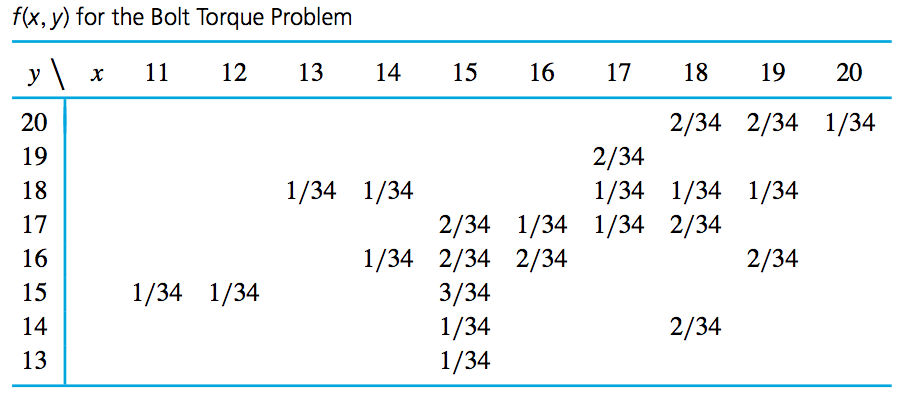
\includegraphics{../../fig/torquetable.png}
\begin{itemize}
\pause \item $P(X = 18 \text{ and } Y = 17) = \frac{2}{34}$
\pause \item $P(X = 14 \text{ and } Y = 19) = 0$
\end{itemize}
\end{frame}

\begin{frame}
\frametitle{Your turn: torque}
\setkeys{Gin}{width=1\textwidth} 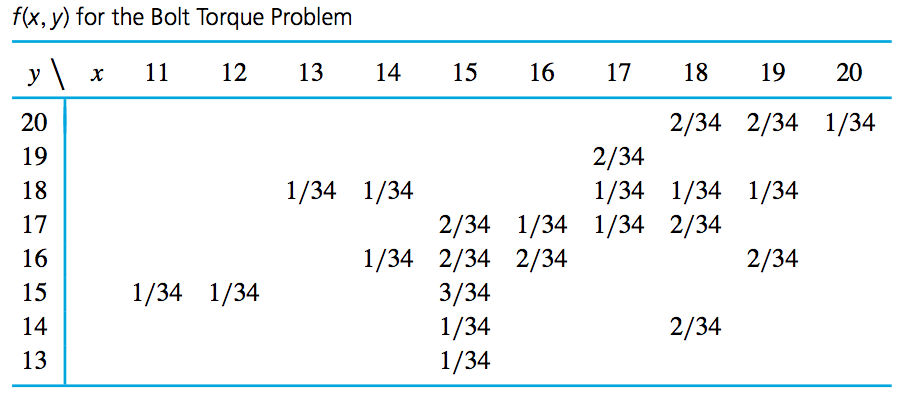
\includegraphics{../../fig/torquetable.png}\q
Calculate:
\begin{enumerate}[1. ]
\item $P(X \ge Y)$
\item $P(|X-Y| \le 1)$
\end{enumerate}
\end{frame}

\begin{frame}<handout:\answers>
\frametitle{Answers: torque} \scriptsize
\setkeys{Gin}{width=.8\textwidth} 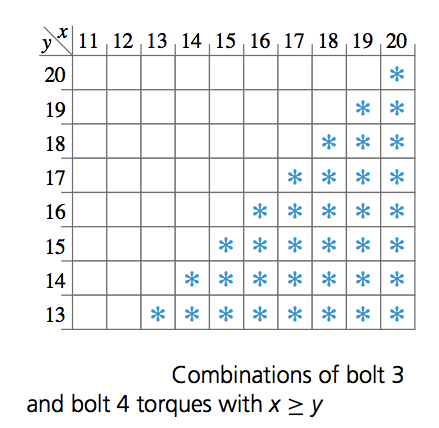
\includegraphics{../../fig/pxlyp.png} 
\end{frame}

\begin{frame}<handout:\answers>
\frametitle{Answers: torque}
\begin{align*}
P(X& \ge Y) = \sum_{x \ge y} f(x, y) \\
&\uncover<2->{= f(20, 20) + f(20, 19) + f(20, 18) + \cdots + f(13, 13)}
\intertext{\uncover<3->{Dropping all the $f(x, y)$ values that equal 0:}}
& \uncover<4->{= f(15, 13) + f(15, 14) + f(15, 15)+ f(16, 16)} \\
& \uncover<4->{ + f(17, 17) + f(18, 14) + f(18, 17) + f(18, 18) } \\
& \uncover<4->{+ f(19, 16) + f(19, 18)+ f(20, 20)} \\
&\uncover<5->{\frac{1}{34} + \frac{1}{34} + \frac{3}{34} + \frac{2}{34} + \cdots + \frac{1}{34}} \uncover<6->{= \frac{17}{34}}
\end{align*}
\end{frame}

\begin{frame}<handout:\answers>
\frametitle{Answers: torque}
\setkeys{Gin}{width=.8\textwidth} 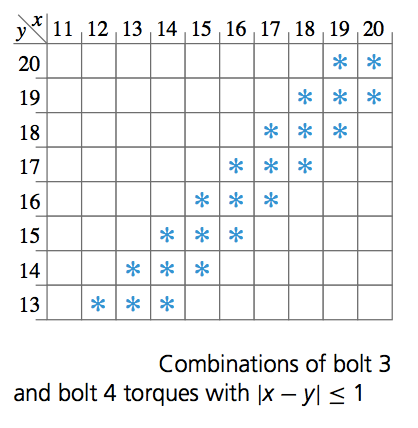
\includegraphics{../../fig/pxy1p.png}
\end{frame}

\begin{frame}<handout:\answers>
\frametitle{Answers: torque} \scriptsize

\begin{align*}
P(X& \ge Y) = \sum_{x \ge y} f(x, y) \\
&\uncover<2->{= f(13, 13) + f(14, 13) + f(14, 14) + \cdots + f(20, 20)}
\intertext{\uncover<3->{Dropping all the $f(x, y)$ values that equal 0:}}
& \uncover<4->{= f(15, 14) + f(15, 15) + f(15, 16)+ f(16, 16)} \\
& \uncover<4->{ + f(16, 17) + f(17, 17) + f(17, 18) + f(18, 17) } \\
& \uncover<4->{+ f(18, 18) + f(19, 18)+ f(19, 20) +  f(20, 20)} \\
&\uncover<5->{= \frac{18}{34}}
\end{align*}
\end{frame}

\subsection{Marginal Distributions}


\begin{frame}
\frametitle{Marginal distributions}
\begin{itemize}
\pause \item The {\bf marginal distributions} of $X$ and $Y$, which have joint pmf $f(x,y)$, are:
\begin{align*}
\uncover<3->{f_X(x) = \sum_y f(x,y)} \\
\uncover<4->{f_Y(y) = \sum_x f(x,y)}
\end{align*}
\uncover<5->{\item $f_X(x)$ is just the ordinary, univariate pmf of $X$.}
\end{itemize}
\end{frame}

\begin{frame}
\frametitle{Your turn: torque}
\begin{itemize}
\item Calculate the marginal pmfs of $X$ and $Y$
\end{itemize}
\setkeys{Gin}{width=1\textwidth} 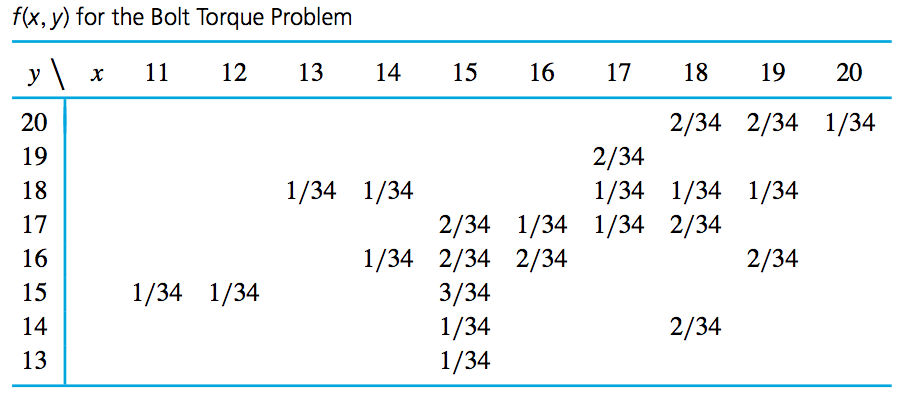
\includegraphics{../../fig/torquetable.png}
\end{frame}

\begin{frame}<handout:\answers>
\frametitle{Answers: torque}
\begin{itemize}
\pause \item Take the column sums to calculate $f_X$ at each $x$.
\pause \item Take the row sums to calculate $f_Y$ at each $y$. 
\end{itemize}
\begin{center}
\pause \begin{tabular}{cc}
$x$ & $f_X(x)$  \\ \hline
11 & 1/34 \\ 
12 & 1/34 \\ 
13 & 1/34 \\ 
14 & 2/34 \\ 
15 & 9/34 \\ 
16 & 3/34 \\ 
17 & 4/34 \\ 
18 & 7/34 \\ 
19 & 5/34 \\ 
20 & 1/34 \\ 
\end{tabular} $\quad$ \begin{tabular}{cc}
$y$ & $f_Y(y)$ \\ \hline
13 & 5/34 \\ 
14 & 2/34 \\ 
15 & 5/34 \\ 
16 & 6/34 \\ 
17 & 7/34 \\ 
18 & 7/34 \\ 
19 & 3/34 \\ 
20 & 1/34 \\ 
{ } & { } \\
{} & {} \\
\end{tabular}
\end{center}
\end{frame}


\begin{frame}<handout:\answers>
\frametitle{Answers: torque}
\begin{itemize}
\item It is customary to write the marginal pmfs in the margins of the table of the joint pmf.
\end{itemize}
\setkeys{Gin}{width=1\textwidth} 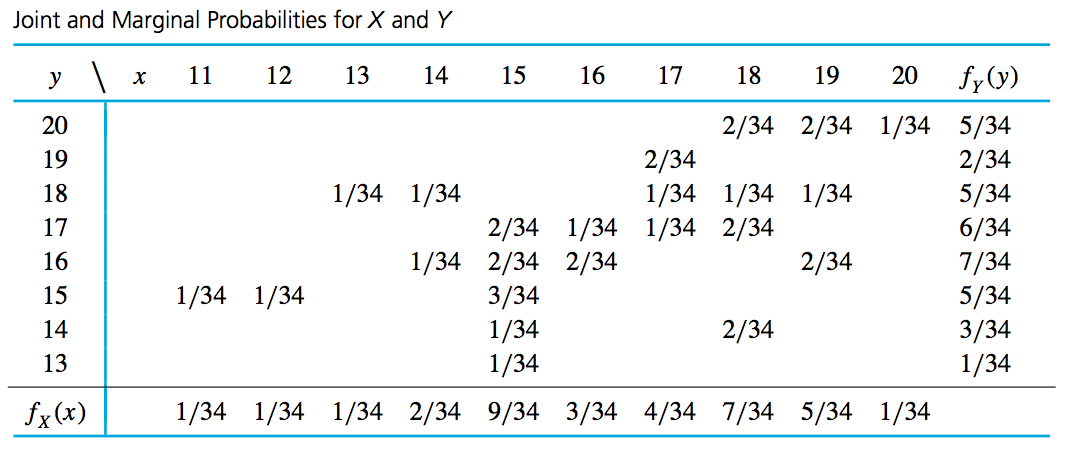
\includegraphics{../../fig/torquetablemar.png}
\end{frame}


\subsection{Conditional Distributions}

\begin{frame}
\frametitle{Conditional distributions}
\begin{itemize}
\pause \item The {\bf conditional distribution} of $Y$ given $X = x$ is a function, $f_{Y \mid X = x}$, given by:
\pause \begin{align*}
f_{Y \mid X = x}(y) = \frac{f(x,y)}{f_X(x)}
\end{align*}
\pause \item To make sense of conditional distributions, return to the torque example...
\end{itemize}
\end{frame}


\begin{frame}
\frametitle{Example: torque} \small
\setkeys{Gin}{width=1\textwidth} 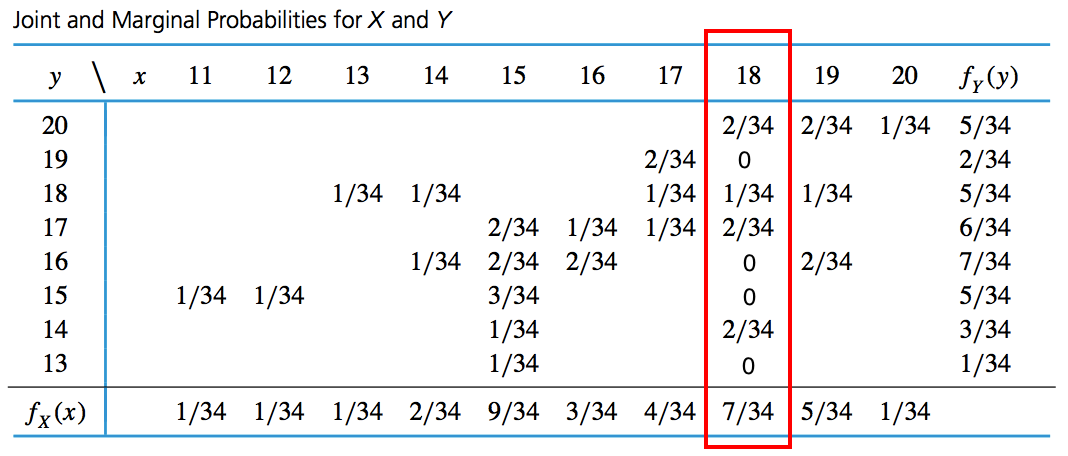
\includegraphics{../../fig/torquetablemar2.png}
\begin{itemize}
\pause \item For example, $f_{Y \mid X = 18}(20) = \frac{2/34}{7/34} = 2/7$. That makes sense because:
\begin{itemize}
\pause \item Since $f_{X}(18) = 7/34$, we expect roughly 7 out of every 34 cases to have $X = 18$.
\pause \item Since $f_{X, Y}(18, 20) = 2/34$, we expect roughly 2 of those 7 cases to also have $Y = 20$.
\end{itemize}
\end{itemize}
\end{frame}

\begin{frame}
\frametitle{Example: torque} \small
\begin{tabular}{ccccccccccc}
$y$ & 13 & 14 & 15 & 16 & 17 & 18 & 19 & 20 \\ \hline
$f_{X, Y}(18, y)$ & 2/34 & 0 & 1/34 & 2/34 & 0 & 0 & 2/34 & 0 \\
$f_{Y \mid X = 18}(y)$ & 2/7 & 0 & 1/7 & 2/7 & 0 & 0 & 2/7 & 0
\end{tabular} \q
\begin{itemize}
\pause \item $\sum_{y = 13}^{20} f_{X, Y}(18, y) = f_{X}(18) = 7/34$ 
\pause \item $\sum_{y = 13}^{20}f_{Y \mid X = 18}(y) = 1$
\pause \item The conditional distribution, $f_{Y \mid X = 18}$ is the renormalized column of the joint distribution corresponding to $X = 18$.
\end{itemize}
\end{frame}

\begin{frame}
\frametitle{Your turn: torque}
\setkeys{Gin}{width=1\textwidth} 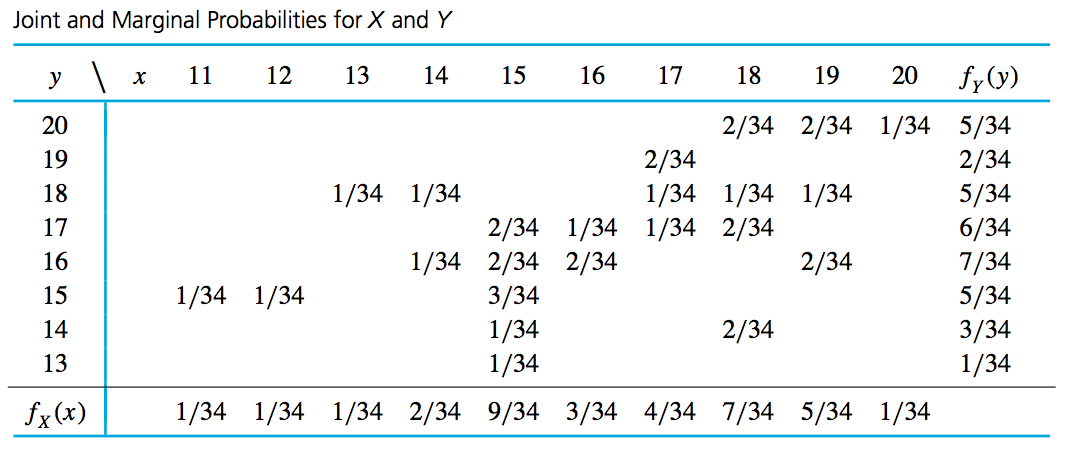
\includegraphics{../../fig/torquetablemar.png}
\begin{itemize}
\item Calculate:
\begin{enumerate}[1. ]
\item $f_{Y \mid X = 15}(y)$
\item $f_{Y \mid X = 20}(y)$
\item $f_{X \mid Y = 18}(x)$
\end{enumerate}
\end{itemize}
\end{frame}

\begin{frame}<handout:\answers>
\frametitle{Answers: torque} \scriptsize
\begin{enumerate}[1. ]
\item 
\begin{tabular}{ccccccccccc}
$y$ & 13 & 14 & 15 & 16 & 17 & 18 & 19 & 20 \\ \hline
$f_{Y \mid X = 15}(y)$ & 1/9 & 1/9 & 3/9 & 2/9 & 2/9 & 0 & 0 & 0
\end{tabular} \q
\item 
\begin{tabular}{ccccccccccc}
$y$ & 13 & 14 & 15 & 16 & 17 & 18 & 19 & 20 \\ \hline
$f_{Y \mid X = 20}(y)$ & 0 & 0 & 0 & 0 & 0 & 0 & 0 & 1
\end{tabular} \q
\item 
\begin{tabular}{ccccccccccccc}
$x$ & 11 & 12 & 13 & 14 & 15 & 16 & 17 & 18 & 19 & 20 \\ \hline
$f_{X \mid Y = 18}(x)$ & 0 & 0 & 1/5 & 1/5 & 0 & 0 & 1/5 & 1/5 & 1/5 & 0
\end{tabular} \q
\end{enumerate}
\end{frame}



\subsection{Independence}

\begin{frame}
\frametitle{\small Given a set of marginal distributions, there are many possible joint distributions.}
\begin{itemize}
\item What do you notice about each of the following joint distributions?
\end{itemize}
\setkeys{Gin}{width=1\textwidth} 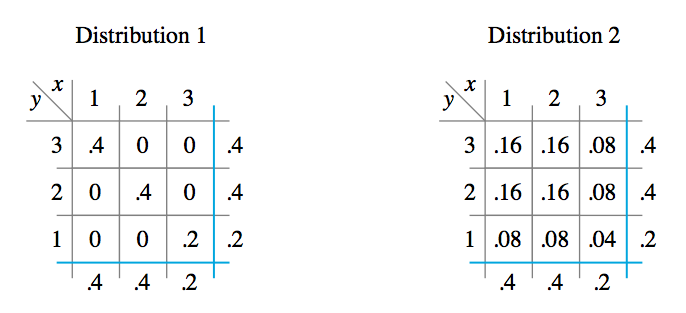
\includegraphics{../../fig/2joint.png}
\end{frame}

\begin{frame}
\frametitle{\small Given a set of marginal distributions, there are many possible joint distributions.} \small
\begin{itemize}
\item What do you notice about each of the following joint distributions?
\end{itemize}
\setkeys{Gin}{width=1\textwidth} 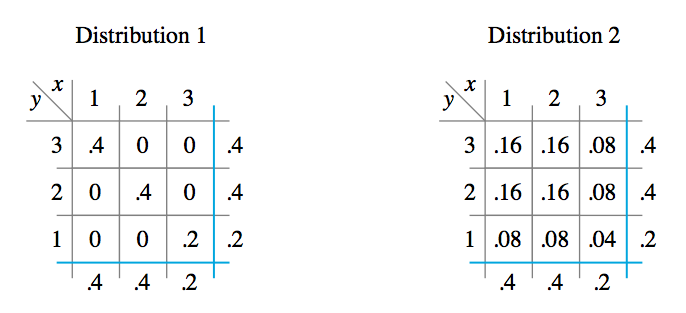
\includegraphics{../../fig/2joint.png}
\begin{enumerate}[1. ]
\pause \item Given $X = x$, you know what $Y$ has to be (and vice versa). 
\pause \item Each $P(X = x, Y = y)$ is just $P(X = x) \cdot P(Y = y)$; i.e., $X$ and $Y$ have no influence on each other.
\end{enumerate}
\end{frame}

\begin{frame}
\frametitle{A look at distribution 2}
\begin{center}
\setkeys{Gin}{width=.4\textwidth} 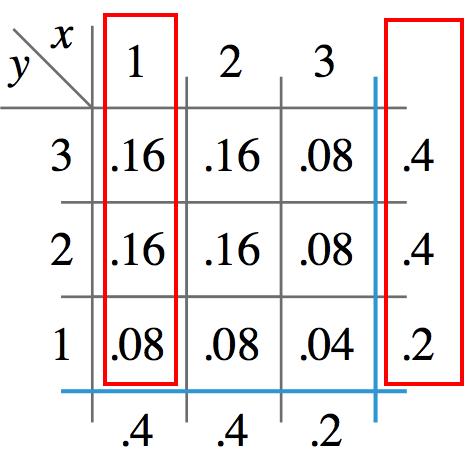
\includegraphics{../../fig/d2.png}
\end{center}
\begin{itemize}
\pause \item Among just the cases when $X = 1$:
\begin{itemize}
\pause \item $Y = 3$ every $16$ out of (16 + 16+ 8) = 40 times: i.e., with probability $\frac{16}{40} = 0.4$ 
\pause \item Same with $Y = 2$
\pause \item $Y = 1$ every $8$ out of (16 + 16+ 8) = 40 times: i.e., with probability 0.2
\end{itemize}
\pause \item So pmf of $Y$ given $X = 1$ is the same as the marginal pmf of $Y$.
\end{itemize}
\end{frame}

\begin{frame}
\frametitle{Independence}
\begin{itemize}
\pause \item Discrete random variables $X$ and $Y$ are independent (written $X \ind Y$) if for all $x$ and $y$,
\pause \begin{align*}
P(Y = y \mid X = x) = P(Y = y) 
\end{align*}
where $\mid$ means ``given".
\pause \item If $X \ind Y$, then:
\begin{align*}
\uncover<5->{P(Y = y \text{ and } X = x)} & \uncover<5->{= P(X = x) \cdot P(Y = y)} \\
\uncover<6->{f(x, y)} & \uncover<6->{= f_X(x) \cdot f_Y(y)}
\end{align*}
\uncover<7->{\item If $X$ and $Y$ are not only independent but also have the same marginal distribution, then they are {\bf independent and identically distributed}, abbreviated {\bf iid}.}
\end{itemize}
\end{frame}

\section{The Continuous Case}

\begin{frame}
\frametitle{Continuous joint distributions}
\begin{itemize}
\pause \item A {\bf joint probability density function} (pdf) for two continuous random variables $X$ and $Y$ is a nonnegative function with:
\begin{align*}
\uncover<3->{\int \int f(x,y) dx dy} & \uncover<3->{= 1} \\
\uncover<4->{P((X, Y) \in R)} & \uncover<4->{= \int \int_R f(x,y) dx dy}
\end{align*}
\uncover<4->{where $R$ is some region of $\mathbb{R}^2$. }
\end{itemize}
\end{frame}



\begin{frame}
\frametitle{Example: sales desk}
\begin{itemize}
\pause \item $S = $ true excess time (over a 7.5 s threshold) required to complete the next sale
\pause \item $R = $ excess time measured with a stopwatch
\end{itemize}

\pause \begin{align*}
f(s,r ) = \begin{cases}
\frac{1}{16.5} e^{-s/16.5} \frac{1}{\sqrt{2 \pi (0.25)}} e^{-(r - s)^2/2(0.25)} & \quad s > 0 \\
0 & \quad \text{otherwise}
\end{cases}
\end{align*}
\end{frame}

\begin{frame}
\frametitle{$f(s, r)$ is valid.} \scriptsize

\begin{align*}
\int \int f(s, r) ds \ dr &= \int_0^\infty \int_{-\infty}^\infty \frac{1}{16.5 \sqrt{2 \pi (0.25)}} e^{-(s/16.5) - ((r-s)^2/2(0.25))} dr \ ds \\
& \uncover<2->{= \int_0^\infty \frac{1}{1.65} e^{-s/16.5} \left \{ \int_{-\infty}^\infty \frac{1}{\sqrt{2 \pi (0.25)}} e^{-(r-s)^2/2(0.25)} dr \right \} ds} \\
&\uncover<3->{= \int_0^\infty \frac{1}{16.5} e^{-s/16.5} ds} \\
&\uncover<4->{= 1}
\end{align*}
\end{frame}

\begin{frame}
\frametitle{A look at $f(s,r)$}
\setkeys{Gin}{width=1\textwidth} 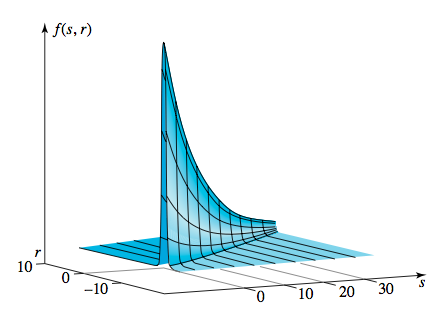
\includegraphics{../../fig/salespict.png}
\end{frame}

\begin{frame}
\frametitle{\small Checking for measurement bias: P(measured excess time $>$ actual excess time)} \scriptsize
\begin{align*}
P(R > S) &= \int \int_{r > s} f(s, r) ds \ dr  \\
&\uncover<2->{= \int_0^\infty \int_s^\infty f(s,r) dr \ ds } \\
&\uncover<3->{= \int_0^\infty \frac{1}{16.5} e^{-s/16.5} \left \{ \int_{s}^\infty \frac{1}{\sqrt{2 \pi (0.25}} e^{-(r-s)^2/2(0.25)} dr \right \} ds} \\
&\uncover<4->{=\int_0^\infty \frac{1}{16.5} e^{-s/16.5} \left \{ \frac{1}{2} \right \} ds} \\
&\uncover<5->{=\frac{1}{2}}
\end{align*}
\end{frame}

\begin{frame}
\frametitle{Checking for measurement bias: region of integration}
\setkeys{Gin}{width=.8\textwidth} 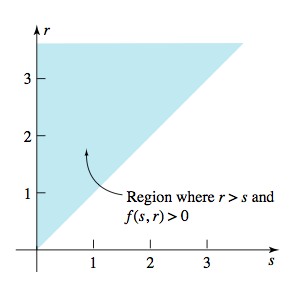
\includegraphics{../../fig/intregion1.png}
\end{frame}

\begin{frame}
\frametitle{Probability of taking too long} \scriptsize
\begin{align*}
P(S > 20) &= \int \int_{s > 20} f(s, r) dr \ ds \\
&\uncover<2->{= \int_{20}^\infty \int_{-\infty}^\infty f(s, r) dr \ ds} \\
&\uncover<3->{=\int_{20}^\infty \frac{1}{16.5} e^{-s/16.5} \left \{\int_{-\infty}^\infty \frac{1}{\sqrt{2 \pi (0.25)}} e^{-(r-s)^2/s(0.25)} \right \} ds} \\
&\uncover<4->{=\int_{20}^\infty e^{-s/16.5} ds} \\
&\uncover<5->{=e^{-20/16.5}} \\
&\uncover<6->{\approx 0.30}
\end{align*}
\end{frame}

\begin{frame}
\frametitle{Probability of taking too long: region of integration}
\setkeys{Gin}{width=.8\textwidth} 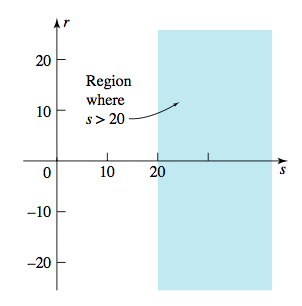
\includegraphics{../../fig/intregion2.png}
\end{frame}

\begin{frame}
\frametitle{Continuous marginal and conditional distributions}
\begin{itemize}
\pause \item For continuous random variables $X$ and $Y$, the {\bf marginal distribution} of $X$ is:
\pause \begin{align*}
f_X(x) = \int_{-\infty}^\infty f(x,y) dy
\end{align*}
\pause \item The {\bf conditional distribution} of $Y$ given $X = x$ is:
\pause \begin{align*}
f_{Y \mid X = x}(y) = \frac{f(x,y)}{f_X(x)}
\end{align*}
\end{itemize}
\end{frame}


\end{document}
